
As mentioned in the introduction, it is usually the case that
after constructing a SSM, the result is a family of models
indexed by the static parameter $\Th$. The ultimate interest might lie in estimating
the states or the parameter or both. Be as it may, the two inference problems are intimately
coupled and interest in the other requires the resolution of the other.

In general, parameter estimation techniques are divided
into offline or \emph{batch} methods and online or \emph{recursive} methods
\parencite{Cappe2007,Kantas2009}. This is analogous to the difference between the filtering and 
smoothing problems in state estimation. We focus only on offline methods, where some 
sort of training or calibration data has been acquired beforehand.

A classic solution to the parameter estimation problem is to introduce
an augmented and necessarily nonlinear SSM, where the parameters have been concatenated as part of the
state. For static parameters, the part of the dynamic model corresponding to the parameters is
set to identity. Classically an extended Kalman filter is 
then applied to approximate the probability distribution of the augmented state
vector in the joint space of parameters and states. This approach is known
as \emph{joint EKF} and it has the virtue of being an online procedure \parencite{Wan2001}.
It appears that the method has problems with convergence in some situations.
A more recent method utilizing another form of augmented SSM is known as \emph{iterated filtering}
\parencite{Ionides2011}. It is an offline method, but only requires being able
to sample from the dynamic model given the parameter and no gradient computations
are required. The algorithm however introduces multiple parameters of its own
and so might require some tuning \parencite{Kantas2009}. Furthermore, it is designed
to utilize the simulation based SMC methods mentioned briefly in Section~\ref{sec:nonlinear_state}.
In the sequel, these kinds of filtering based parameter estimation methods 
will not be further considered. 


% Let us then concern ourselves for a moment with the difference between the states
% and the parameters in a SSM. In the introduction it was stated that in this
% thesis the distinction is that the states are dynamic and the parameters are
% static. But this is only true in the sense that for the states a probability
% distribution is computed for every timestep. The marginal distribution
% of the static components could still be static.
% Thus the SSM of equation~\eqref{eq:ssm_too_general}
% could be reformulated by augmenting $\Th$ as part of the state and
% modifying $\ff$ and $\hh$ accordingly. In this
% way a separate parameter estimation problem would not exist.
% Parameter estimation by state augmentation is known as  


%%%%%%%%%%%%%%%%%%%%%%%%%%%%%%%%%%%%%%%%%%%%%%%%%%%%%%%%%%%%%%%%%%%%%%%%%
\subsection{Bayesian Estimation of Parameters}%%%%%%
%%%%%%%%%%%%%%%%%%%%%%%%%%%%%%%%%%%%%%%%%%%%%%%%%%%%%%%%%%%%%%%%%%%%%%%%%
In the Bayesian sense the complete 
answer to the filtering and parameter estimation problems would be the \emph{joint} posterior distribution of the states
and the parameters given the data
\begin{align}
	% \Pdf{\X,\Th}{\Y}\propto\frac{\Pdf{\X,\Y}{\Th}}{\Pdf{\Y}{\Th}}\frac{\Pdf{\Y}{\Th}\Pdf{\Th}}{\defint{\Theta}{}{\Pdf{\Y}{\Th}\Pdf{\Th}}{\Th}}
	\Pdf{\X,\Th}{\Y} &\propto \Pdf{\X,\Y}{\Th}\Pdf{\Th}\\
	&= \Pdf{\X}{\Y,\Th}\Pdf{\Y}{\Th}\Pdf{\Th}
	\label{eq:param_post}
\end{align}
By defining the SSM in Equation~\eqref{eq:ssm_general}, we have
implicitly defined the ``complete-data'' likelihood $\Pdf{\X,\Y}{\Th}$
(see Equation~\eqref{eq:complete_data_likelihood}).
By introducing the \emph{prior distribution}, $\Pdf{\Th}$,
the components of \eqref{eq:param_post} and thus the joint distribution posterior
of states and parametes is defined. Recently, methods known as
\emph{Particle Markov chain Monte Carlo} (PMCMC) have emerged,
which are able to sample from the joint distribution in \eqref{eq:param_post}
without knowledge of the normalization constant \parencite{Andrieu2010}.
This is achieved by combining particle filtering approximations to $\Pdf{\X}{\Y,\Th}$ 
with traditional Gibbs and Metropolis-Hastings sampling in a nontrivial way 
\parencite{Andrieu2010,gelman2004}.

\subsubsection{Maximum a posteriori and maximum likelihood}

In this thesis we would like to avoid Monte Carlo methods altogether. Thus instead
of considering the problem of finding the posterior distribution of the parameter,
we will pursue finding the mode of this distribution, that is, the \emph{maximum a posteriori} (MAP) estimate
$\Th_{\text{MAP}}$. The MAP estimate is not necessarily unique. 
We will consider the uniqueness issue later in more detail, but in order
to not get distracted, let us assume for the moment that the posterior distribution in fact
has a unique maximum. Since the logarithm is a strictly monotonic function, maximizing a function
is the same as maximizing its logarithm. 
Since $\Y$ is observed, let us denote 
the log marginal likelihood with 
\begin{align*}
	\lLH \equiv \log \Pdf{\Y}{\Th}.
\end{align*}
The MAP estimate of $\Th$ is then defined as 
\begin{align}
	\Th_{\text{MAP}} &\equiv \argmax_{\Th}\brak[\big]{ \log\Pdf{\Th}{\Y}} \nonumber\\ 
	&=\argmax_{\Th}\brak[\big]{\lLH + \log\Pdf{\Th}+C}, && \text{($C$ is independent of $\Th$)} \nonumber\\
	&=\argmax_{\Th}\brak[\big]{\lLH + \log\Pdf{\Th}}\\
	%&=\argmin_{\Th}\brak[\big]{\ene},
	\label{eq:MAP}
\end{align}
\todo{explain the uses of the MAP estimate from Gelman}
%The MAP estimate might be used as is in order to obtain a state estimates
%with supposedly probable parameter values. It could also be used as the initial
%value for simulation based approaches or to compare results obtained with other
%methods.

In the case of a uniform (constant and thus improper)
prior distribution, $\Pdf{\Th}=C$, the MAP estimate reduces to the
\emph{maximum likelihood} (ML) estimate
\begin{align}
	\Th_{\text{ML}} &\equiv \argmax_{\Th}\brak[\big]\lLH\label{eq:ML}
\end{align}
In the limit of infinite data, the influence of the prior
disappears. Then if the support of the prior includes the true
parameter value, the MAP estimate has the same asymptotic properties
as the ML estimate \parencite{Cappe2005}. These properties will be discussed in more
detail in Section~\ref{sec:theory}. Since the mathematical difference
between the MAP and ML estimates depends only on the model dependent prior distribution
assigned to $\Th$, we will mainly focus on computing the ML estimate.
Some steps where the prior plays an important role will be separately
highlighted. 

With the help of the Gaussian filtering and smoothing methodology introduced in 
Section~\ref{sec:nonlinear_state}, computing the (approximate) MAP estimate 
corresponds to maximizing a completely known function.
Thus the problem is turned into one of nonlinear optimization 
(also called nonlinear programming) \parencite{Cappe2005}.

\subsubsection{Ascent methods}

Both of the parameter estimation methods we are going
discuss, the expectation maximization algorithm and
the instances of gradient based nonlinear programming dealt with in the
next chapter, belong to the class of \emph{iterative ascent methods} \parencite{luenberger2008}.
Suppose that $\v{m}:\Theta \to \Theta$ defines an iterative ascent method
and that we are maximizing the objective function $\varphi:\Theta\to\R$.
Then given some initial point $\Th_0$, the sequence of estimates
$\brac{\Th_j \in \Theta: \Th_j=\v{m}(\Th_{j-1})}$ where $j=1,\dots$
has the property $\varphi(\Th_{j})\geq \varphi(\Th_{j-1})$. This means
that the objective function is increased at every iteration of
an iterative ascent method.

%%%%%%%%%%%%%%%%%%%%%%%%%%%%%%%%%%%%%%%%%%%%%%%%%%%%%%%%%%%%%%%%%%%%%
\subsection{Gradient based nonlinear optimization}\label{sec:grad}%%%
%%%%%%%%%%%%%%%%%%%%%%%%%%%%%%%%%%%%%%%%%%%%%%%%%%%%%%%%%%%%%%%%%%%%%

There exists a large amount of efficient nonlinear optimization,
also called nonlinear programming, methods that require the gradient of the 
objective function to be available \parencite{luenberger2008}.
The best known general purpose algorithms probably belong to the 
classes of quasi-Newton or conjugate gradient methods. 
For example, MATLAB Optimization Toolbox contains the function
\texttt{fminunc} utilizing both conjugate gradient and 
quasi-Newton methods in certain cases \parencite{optimizationtoolbox2012}.

The simplest gradient based method is the \emph{method of steepest ascent}.
It requires that the first partial derivatives of the objective function are defined
and continuous in their domain. The method of steepest ascent is then defined
by the iteration
\begin{align}
	\Th_{j+1}&=\Th_j+\alpha_j\nabla\lLH[\Th_j].
	\label{eq:steepest_descent}
\end{align}
The idea is intuitive since it is well known that the gradient
points to the direction of steepest ascent, i.e. to the direction
that is orthogonal to the isolines of constant value.
To determine $\alpha_j$, the \emph{step size}, another minimization problem needs to be solved,
namely
\begin{align}
	\alpha_j &= \argmin_\alpha \lLH[\Th_j+\alpha\nabla\lLH[\Th_j]].
	\label{eq:line_search}
\end{align}
These one dimensional optimization algorithms that are used
to solve the step-sizes are known as \emph{line search} methods \parencite{luenberger2008}.
Common line search methods include the golden rule method and 
methods based on polynomial interpolation.

We define the \emph{order of convergence} as the supremum of the
numbers $p\geq 0$, where
\begin{align}
	0\geq \bar{\lim_{j\to\infty}}\frac{\abs{\Th_{j+1}-\Th_\star}}{\abs{\Th_{j}-\Th_\star}^p} < \infty.
	\label{eq:order_of_convergence}
\end{align}
When $p=1$, we also define the \emph{linear rate of convergence} as
the number $0 \leq \rho < 1$ in
\begin{align}
	\lim_{j\to\infty}\frac{\abs{\Th_{j+1}-\Th_\star}}{\abs{\Th_{j}-\Th_\star}} = \rho.
	\label{eq:rate_of_convergence}
\end{align}
It can be shown the steepest ascent method has linear order of convergence ($p=1$)
and if the Hessian of the objective function is positive definite with
$r=A/a$, the ratio of the largest and smallest eigenvalues, 
\begin{align}
	\lim_{j\to\infty}\frac{\abs{\Th_{j+1}-\Th_\star}}{\abs{\Th_{j}-\Th_\star}} \leq \left(\frac{r-1}{r+1}\right)^2.
\end{align}
A much more efficient nonlinear optimization algorithm is the \emph{Newton's method}.
It is based on Taylor expanding the objective function around the
current estimate $\Th_j$. Assume that $\ell$ has continuous second-order partial derivatives. Then
\begin{align}
	\lLH[\Th] &\approx \lLH[\Th_j]+\nabla\lLH[\Th_j]^\tr\fparen*{\Th_j-\Th}+\frac{1}{2}\fparen*{\Th_j-\Th}^\tr\nabla^2\lLH[\Th_j]\fparen*{\Th_j-\Th}
	\label{eq:second_order_expansion}
\end{align}
and then maximizing the approximation by setting its gradient to zero
\begin{align}
	\nabla\lLH[\Th_j]-\nabla^2\lLH[\Th_j]\fparen*{\Th_j-\Th} &= 0\\
	\Rightarrow \Th_{j+1} &= \Th_j+\nabla^2\lLH[\Th_j]^{-1}\nabla\lLH[\Th_j].
	\label{eq:newton_gradient}
\end{align}
Per proposition~\ref{prop:cond_for_max}, near $\Th_\star$ the Hessian is 
invertible and so the algorithm is well defined there. It can be shown
that when initialized sufficiently close to $\Th_\star$, (pure form)
Newton's method always converges to $\Th_\star$ with order of convergence
at least \emph{two}.
 
Further away from the maximum, there are various problems with Newton's method as formulated
in equation~\eqref{eq:newton_gradient}. There are no guarantees for the invertibility
of the Hessian and higher order terms may cause a step to actually decrease the objective
function. Thus we turn our attention to algorithms of the general form
\begin{align}
	\Th_{j+1} &= \Th_j+\alpha_j\v{D}_j\nabla\lLH[\Th_j],
	\label{eq:gradient_method_general}
\end{align}
where $\v{D}_j$ is a symmetric matrix, the \emph{search direction} is $\v{D}_j\nabla\lLH[\Th_j]$ and
the step-size is $\alpha_j$. Generally $\v{D}_j$ should also be negative definite, to guarantee
that the method is an ascent method for small $\alpha_j$ (as in proposition \eqref{prop:cond_for_max}).
  
Clearly we get gradient ascent with $\v{D}_j=\v{I}$
and Newton's method with  $\v{D}_j=\nabla^2\lLH[\Th_j]^{-1}$. 
Other methods of this form have thus orders of convergence
between one and two. In practice the step
size parameter is always determined by a line-search, so that different
algorithms of the form \eqref{eq:gradient_method_general} differ only in how
the search direction is computed. Even if we could guarantee the invertability of the Hessian, its computation is
nevertheless notoriously computationally demanding. 

Thus we will discuss methods derived from Newton's method, but which only require
gradient information. These are commonly known as \emph{quasi-Newton} methods or 
sometimes \emph{secant methods} \parencite{Battiti1992}. Given the analytical gradient, 
the idea is to \emph{iteratively} approximate the analytical inverse Hessian by utilizing
the information gathered as the ascent method advances. Suppose we are given
two points $\Th_{j}$ and $\Th_{j+1}$ and that
\begin{align}
	\g_j &\equiv \nabla\lLH[\Th_j]\\
	\q_j &\equiv \g_{j+1}-\g_j\\
	\p_k &\equiv \Th_{j+1}-\Th_j.
\end{align}  
We could then approximate the Hessian with
\begin{align}
	\q_j &\approx \nabla^2\lLH[\Th_j] \p_j,
	\label{eq:secant_approx}
\end{align}
which in the one dimensional case is the slope of the secant line drawn 
through the two points $\theta_1$ and $\theta_2$.
In case of constant Hessian, equation~\eqref{eq:secant_approx} becomes exact.
In multiple dimensions equation~\ref{eq:secant_approx} doesn't give a unique solution for
the approximate Hessian. The Broyden \emph{update} suggests to pick the one
that deviates the least from the current approximation in the sense of the Frobenius norm.
Let us suppose that we're searching for a symmetric and negative definite approximate Hessian
$\widehat{\v{H}}_{j+1}$ based on the current approximation $\widehat{\v{H}}_{j}$.
Since the Broyden update doesn't guarantee negative definiteness we instead update 
an \emph{invertible} Cholesky factor, thus guaranteeing the negative-definiteness of $\widehat{\v{H}}_{j+1}$.
These considerations lead to the widely applied \emph{Broyden-Fletcher-Goldfarb-Shanno} (BFGS) \parencite{BROYDEN01121973,Battiti1992} update
\begin{align}
	\widehat{\v{H}}_{j+1}=\widehat{\v{H}}_{j}+\frac{\q_k\q_k^\tr}{\q_k^\tr\p_k}+\frac{\widehat{\v{H}}_{j}\p_k\p_k^\tr\widehat{\v{H}}_{j}}{\p_k^\tr\widehat{\v{H}}_{j}\p_k}.
\end{align}
Since we are actually in need for the approximate \emph{inverse} Hessian,
applying the Sherman-Morrison inversion formula gives
\begin{align}
	\widehat{\v{H}}_{j+1}^{-1}=\widehat{\v{H}}_{j}^{-1}+\fparen*{\frac{1+\q_k^\tr\widehat{\v{H}}_{j}^{-1}\q_k}{\q_k^\tr\q_k}}\frac{\p_k\p_k^\tr}{\p_k^\tr\q_k}+
	\frac{\p_k\q_k^\tr\widehat{\v{H}}^{-1}_{j}+\widehat{\v{H}}^{-1}_{j}\q_k\q_k^\tr}{\q_k^\tr\p_k}.
\end{align}
It should be pointed that the commonly used MATLAB unconditional nonlinear
optimization function \texttt{fminunc} that we referred to earlier, uses 
the BFGS quasi-Newton method with cubic interpolation line search.

\subsubsection{Linear-Gaussian SSMs}\label{sec:grad_LGSSM}

Let us then focus on computing the gradient of the
log-likelihood function $\lLH$, also known as the \emph{score function}.
By marginalizing the joint distribution of equation~\eqref{eq:joint_per_kalmanstep}
we get 
\begin{align}
	\Pdf{\y_k}{\y_{1:k-1},\Th}&=\N[\yk]{\v{H}\m_{k|k-1},\v{S}_k }.
\end{align}
Applying equation~\eqref{eq:lh_factorization} and taking the logarithm then gives
\begin{align}
	\lLH&=-\frac{1}{2}\sum_{k=1}^T\log\det{\v{S}_k}
	-\frac{1}{2}\sum_{k=1}^T\left(\v{y}_k-\v{H}\v{m}_{k|k-1}\right)^\tr\v{S}_{k}^{-1}\left(\v{y}_k-\v{H}\v{m}_{k|k-1}\right)+C,
	\label{eq:logLH}
\end{align}
where $C$ is a constant that doesn't depend on $\gv{\theta}$ and thus can
be ignored in the maximization.
There are exists two seemingly quite different methods for computing
the gradient of $\lLH$. The first one proceeds straightforwardly by taking the
partial derivatives of $\lLH$. As will soon be demonstrated, this leads
to some additional recursive formulas which allow computing
the gradient in parallel with the Kalman filter. The second method needs
the smoothing distributions with the cross-timestep covariances
and it can be easily computed with the expectation maximization machinery
that will be introduced later. These two methods can be proved to compute
the exact same quantity. At this point we will focus on the first one. Going further
it will be assumed that $\lLH$ is continuous and differentiable for all $\Th\in\Theta$.

In order to calculate the score function
\begin{align}
	\score[\Th']&=\eval{\dpd{\lLH}{\Th}}_{\Th=\Th'}
	=\eval{\bm{\dpd{\lLH}{\theta_1} & \dots & \dpd{\lLH}{\theta_{d_\theta}}}^\tr}_{\Th=\Th'},
	\label{eq:score}
\end{align}
we have to compute the partial
derivatives:
\begin{align}
\begin{split}
	\dpd{\lLH}{\theta_i}
	=&-\frac{1}{2}\sum_{k=1}^T\mathrm{Tr}\left(\v{S}_{k}^{-1}\dpd{\v{S}_k}{\theta_i}\right)\\
	&+\sum_{k=1}^T\left(\v{H}_k\dpd{\v{m}_{k|k-1}}{\theta_i}\right)^\tr\v{S}_{k}^{-1}\left(\v{y}_k-\v{H}\v{m}_{k|k-1}\right)\\
	&+\frac{1}{2}\sum_{k=1}^T\left(\v{y}_k-\v{H}\v{m}_{k|k-1}\right)^\tr\v{S}_{k}^{-1}\left(\dpd{\v{S}_k}{\theta_i}\right)\v{S}_{k}^{-1}\left(\v{y}_k-\v{H}\v{m}_{k|k-1}\right)\\
	\label{eq:dlogLH}
\end{split}
\end{align}
From the Kalman filter recursions \eqref{eq:Kalman_filter} we find out that 
\begin{align}
	\dpd{\v{S}_k}{\theta_i}&=\v{H}\dpd{\v{P}_{k|k-1}}{\theta_i}\v{H}+\dpd{\v{R}}{\theta_i}
\end{align}
so that we're left with the task of determining the partial derivatives for
$\v{m}_{k|k-1}$ and $\v{P}_{k|k-1}$:
\begin{align}
	\dpd{\v{m}_{k|k-1}}{\theta_i}&=\dpd{\v{A}}{\theta_i}\v{m}_{k-1|k-1}+\v{A}\dpd{\v{m}_{k-1|k-1}}{\theta_i} \label{eq:m_pred_pd}\\
	\begin{split}
	\dpd{\v{P}_{k|k-1}}{\theta_i}&=\dpd{\v{A}}{\theta_i}\v{P}_{k-1|k-1}\v{A}^\tr+\v{A}\dpd{\v{P}_{k-1|k-1}}{\theta_i}\v{A}^\tr\\
	&+\v{A}\v{P}_{k-1|k-1}\left(\dpd{\v{A}}{\theta_i}\right)^\tr+\dpd{\v{Q}}{\theta_i} \label{eq:P_pred_pd}
	\end{split}
\end{align}
as well as for $\v{m}_{k|k}$ and $\v{P}_{k|k}$:
\begin{align}
	\dpd{\v{K}_k}{\theta_i}&=\dpd{\v{P}_{k|k-1}}{\theta_i}\v{H}^\tr\v{S}_{k}^{-1}-\v{P}_{k|k-1}\v{H}^\tr\v{S}_{k}^{-1}\dpd{\v{S}_k}{\theta_i}\v{S}_{k}^{-1}
	\label{eq:K_pd}\\
	\dpd{\v{m}_{k|k}}{\theta_i}&=\dpd{\v{m}_{k|k-1}}{\theta_i}+\dpd{\v{K}_k}{\theta_i}\left(\v{y}_k-\v{H}\v{m}_{k|k-1}\right)-\v{K}_k\v{H}\dpd{\v{m}_{k|k-1}}{\theta_i}
	\label{eq:m_pd}\\
	\dpd{\v{P}_{k|k}}{\theta_i}&=\dpd{\v{P}_{k|k-1}}{\theta_i}-\dpd{\v{K}_k}{\theta_i}\v{S}_{k}\v{K}_{k}^\tr-\v{K}_{k}\dpd{\v{S}_k}{\theta_i}\v{K}_{k}^\tr-\v{K}_{k}^\tr\v{S}_{k}\left(\dpd{\v{K}_k}{\theta_i}\right)^\tr
	\label{eq:P_pd}
	\end{align}
Equations \eqref{eq:m_pred_pd}, \eqref{eq:P_pred_pd}, \eqref{eq:K_pd}, \eqref{eq:m_pd} and \eqref{eq:P_pd} together specify
a recursive algorithm for computing \eqref{eq:dlogLH} that can be run alongside the Kalman filter recursions.
As noted in \textcite{Cappe2005}, these equations are sometimes known as the \emph{sensitivity equations}
and they are derived at least in \textcite{Gupta1974}.


%%%%%%%%%%%%%%%%%%%%%%%%%%%%%%%%%%%%%%%%%%%%%%%%%%%%%
\subsubsection{Nonlinear-Gaussian SSMs}%%%%%%%%%%%%%%
%%%%%%%%%%%%%%%%%%%%%%%%%%%%%%%%%%%%%%%%%%%%%%%%%%%%%


Here we will present the derivation of the sensitivity equations for nonlinear SSMs with additive
Gaussian noise. Since the predictive and filtering distributions have to be approximated in the nonlinear
case, we will work in the Gaussian filtering framework. The 3rd order spherical cubature approximation
of Equation~\eqref{eq:ckf_approx} will be applied to integrals intractable in closed form. The result
is an approximate recursive algorithm for computing $\pd{\m_{k|k}}{\theta_i}$ and $\pd{\P_{k|k}}{\theta_i}$,
i.e. the partial derivatives of the mean and and variance of the filtering distributions. These enable
us to compute the partial derivatives of the marginal log-likelihood and by Equation~\eqref{eq:score},
an approximation to the score function.

By marginalizing the joint distribution of equation~\eqref{eq:joint_update_approximation}
we get the approximation
\begin{align}
	\Pdf{\y_k}{\y_{1:k-1},\Th}&\approx \N[\yk]{\gv{\mu}_k,\v{S}_k} ,
\end{align}
so that taking the logarithm of the factorization \eqref{eq:lh_factorization} 
gives the approximate log marginal likelihood 
\begin{align}
	\lLH&\approx
	-\frac{1}{2}\sum_{k=1}^T\log\det{\S}
	-\frac{1}{2}\sum_{k=1}^T
	\left(\yk-\ym\right)^\tr
	\S^{-1}
	\left(\yk-\ym\right),
	\label{eq:nonl_logLH}
\end{align}
where terms independent of $\Th$ have been dropped.
To compute the score function, we need the partial derivatives
\begin{align}
\begin{split}
	\dpd{\lLH}{\theta_i}
	\approx&-\frac{1}{2}\sum_{k=1}^T
	\mathrm{Tr}\left(\S^{-1}\dpd{\S}{\theta_i}\right)\\
	&+\sum_{k=1}^T
	\left(\dpd{\ym}{\theta_i}\right)^\tr\S^{-1}\left(\yk-\ym\right)\\
	&+\frac{1}{2}\sum_{k=1}^T
	\left(\yk-\ym\right)^\tr\S^{-1}\left(\dpd{\S}{\theta_i}\right)\S^{-1}\left(\yk-\ym\right)\\
	\label{eq:nonl_dlogLH}
\end{split}
\end{align}
%
%
Let us denote the predictive distribution sigma points by 
$\sig_{k|k-1}=\m_{k|k-1}+\sqrt{\P_{k|k-1}}\usig$, where $j=1,\dots,2\,d_x$.
For unclutteredness, let us also denote the constant
weight by $w\equiv \sfrac{1}{2d_x}$. Let us first focus on computing
an approximation to 
\begin{align}
	\dpd{\sig_{k|k-1}}{\theta_i}&= \dpd{\m_{k|k-1}}{\theta_i}+ \dpd{\sqrt{\P_{k|k-1}}}{\theta_i}\usig
	\label{eq:dSig_pred}
\end{align}
By applying the cubature rule to the integrals \eqref{eq:prediction_mean_intergral} and 
\eqref{eq:prediction_variance_intergral} 
we get   
%
\begin{align}
	\m_{k|k-1} &\approx{} w \sum_{j=1}^{2\,d_x} \ffi[\big]{\sig_{k-1|k-1}} \\
	\P_{k|k-1} &\approx{} w \sum_{j=1}^{2\,d_x}% 
	\Big(\ffi[\big]{\sig_{k-1|k-1}}-\m_{k|k-1}\Big)%
	\Big(\ffi[\big]{\sig_{k-1|k-1}}-\m_{k|k-1}\Big)^\tr%
	+\v{Q},
	\label{tablelabel}
\end{align}
so that the partial derivatives of these become
\begin{align}
	\dpd{\m_{k|k-1}}{\theta_i} &\approx{} w\sum_{j=1}^{2\,d_x}%
	\jacob{\f}{\sig_{k-1|k-1}}\dpd{\sig_{k-1|k-1}}{\theta_i}
	\label{eq:dmpred_cubature_approx}
\shortintertext{and}
	\dpd{\P_{k|k-1}}{\theta_i} &\approx{} \\
	w\sum_{j=1}^{2\,d_x}\bigg[
	&\Big(\jacob{\f}{\sig_{k-1|k-1}}\dpd{\sig_{k-1|k-1}}{\theta_i}-\dpd{\m_{k|k-1}}{\theta_i}\Big)%
	 \Big(\ffi[\big]{\sig_{k-1|k-1}}-\m_{k|k-1}\Big)^\tr\\
   +&\Big(\ffi[\big]{\sig_{k-1|k-1}}-\m_{k|k-1}\Big)%
	 \Big(\jacob{\f}{\sig_{k-1|k-1}}\dpd{\sig_{k-1|k-1}}{\theta_i}-\dpd{\m_{k|k-1}}{\theta_i}\Big)^\tr\bigg]\\%
   +&\dpd{\v{Q}}{\theta_i}.
	\label{eq:dPpred_cubature_approx}
\end{align}
%
Here $\jacob[\displaysize]{\f}{\cdot}$ denotes the Jacobian of $\f$.
We assume that at the current iteration $k$ we have available the approximate mean and variance of the previous 
filtering distribution, i.e $\m_{k-1|k-1}$ and $\P_{k-1|k-1}$, as well as the  
partial derivatives $\pd{\m_{k-1|k-1}}{\theta_i}$ and $\pd{\P_{k-1|k-1}}{\theta_i}$.
This means we can form $\sig_{k-1|k-1}=\m_{k-1|k-1}+\sqrt{\P_{k-1|k-1}}\usig$. 
 
In  $\pd{\sig_{k|k-1}}{\theta_i}$ we clearly need $\pd{\sqrt{\P_{k|k-1}}}{\theta_i}$,
i.e. the partial derivative of the Cholesky decomposition of $\P_{k|k-1}$. 
Having $\pd{\P_{k|k-1}}{\theta_i}$ available, this can be obtained for example by differentiating
an algorithm for computing the Cholesky decomposition.

Then by applying the cubature rule to the integral \eqref{eq:update_variance_intergral}
we get
\begin{align}
	\S \approx  w \sum_{j=1}^{2\,d_x} 
	\left(\hhi[\big]{\sig_{k|k-1}}-\ym\right)
	\left(\hhi[\big]{\sig_{k|k-1}}-\ym\right)^\tr+\v{R},
	\label{eq:S_cubature_approx}
\end{align} 
so that 
\begin{align}
	\dpd{\S}{\theta_i} \approx{}w \sum_{j=1}^{2\,d_x}\bigg[
	 &\Big(\jacob{\h}{\sig_{k|k-1}}\dpd{\sig_{k|k-1}}{\theta_i}-\dpd{\ym}{\theta_i}\Big)\Big(\hhi[\big]{\sig_{k|k-1}}-\ym\Big)^\tr+\\
	 &\Big(\hhi[\big]{\sig_{k|k-1}}-\ym\Big)\Big(\jacob{\h}{\sig_{k|k-1}}\dpd{\sig_{k|k-1}}{\theta_i}-\dpd{\ym}{\theta_i}\Big)^\tr\bigg]
	+\dpd{\v{R}}{\theta_i},
	\label{eq:dS_cubature_approx}
\end{align}
where $\jacob[\displaysize]{\h}{\cdot}$ denotes the Jacobian of $\h$.
%
The approximate partial derivative of $\ym$ can be derived from Equation~\eqref{eq:update_mean_intergral}:
\begin{align}
	\dpd{\ym}{\theta_i} &\approx{} w\sum_{j=1}^{2\,d_x}\jacob{\h}{\sig_{k|k-1}}\dpd{\sig_{k|k-1}}{\theta_i}.
	\label{eq:dmu_cubature_approx}
\end{align}
%
From Equation~\eqref{eq:kalman_gain_nonl} we get
\begin{align}
	\dpd{\v{K}_{k}}{\theta_i} &=  \dpd{\v{C}_k}{\theta_i}\S^{-1}-\v{C}_k\S^{-1}\dpd{\S}{\theta_i}\S^{-1}
	\label{eq:dK_cubature_approx}
\end{align}
and Equation~\eqref{eq:update_covariance_intergral} gives
\begin{align}
	\v{C}_k \approx  w \sum_{j=1}^{2\,d_x} 
	\left(\sig_{k|k-1}-\m_{k|k-1}\right)
	\left(\hhi[\big]{\sig_{k|k-1}}-\ym\right)^\tr,
	\label{eq:C_cubature_approx}
\end{align} 
so that 
\begin{align}
	\dpd{\v{C}_k}{\theta_i} \approx{} w\sum_{j=1}^{2\,d_x}\bigg[
	&\Big(\dpd{\sig_{k|k-1}}{\theta_i}-\dpd{\m_{k|k-1}}{\theta_i}\Big)\Big(\hhi[\big]{\sig_{k|k-1}}-\ym\Big)^\tr+\\
	&\Big(\sig_{k|k-1}-\m_{k|k-1}\Big)
	\Big(\jacob{\h}{\sig_{k|k-1}}\dpd{\sig_{k|k-1}}{\theta_i}-\dpd{\ym}{\theta_i}\Big)^\tr\bigg].
	\label{eq:dC_cubature_approx}
\end{align}
Finally, from Equations \eqref{eq:mean_update_nonl} and \eqref{eq:variance_update_nonl}
we obtain
\begin{align}
	\dpd{\m_{k|k}}{\theta_i} &=  \dpd{\m_{k|k-1}}{\theta_i}+\dpd{\v{K}_{k}}{\theta_i}\left(\yk
	-\ym\right)-\v{K}_{k}\dpd{\ym}{\theta_i}.
	\label{eq:m_pd_nonl}
\shortintertext{and}
	\dpd{\v{P}_{k|k}}{\theta_i} &= \dpd{\v{P}_{k|k-1}}{\theta_i}-
	\dpd{\v{K}_k}{\theta_i}\S\v{K}_{k}^\tr-\v{K}_{k}\dpd{\S}{\theta_i}\v{K}_{k}^\tr-
	\v{K}_{k}^\tr\S\left(\dpd{\v{K}_k}{\theta_i}\right)^\tr
	\label{eq:P_pd_nonl}
\end{align}


%







% \begin{align}
% \fparen[\big]{\h_k-\gv{\mu}_k}\fparen[\big]{\h_k-\gv{\mu}_k}^\tr
% 
% 	\defint{\mathcal{X}}{}{\F{\gv{\kappa}}{\x}\N[\x]{\m}{\P}}{\x} &\approx 
% 	\frac{1}{2\,d_x} \sum_{i=1}^{2\,d_x} \F{\gv{\kappa}}{\m+\sqrt{\P}\gv{\varepsilon}^{(i)}},
% 	\label{eq:ckf_approx}
% \end{align}%
% 
% \begin{align}
% 	\gv{\varepsilon}^{(i)} &= \sqrt{d_x}\v{e}_i &  i&=1,\dots,d_x\\
% 	\gv{\varepsilon}^{(i)} &= -\sqrt{d_x}\v{e}_{i-d_x} & i&=d_x+1,\dots,2\,d_x,
% 	\label{eq:ckf_sigma}
% \end{align}











%%%%%%%%%%%%%%%%%%%%%%%%%%%%%%%%%%%%%%%%%%%%%%
\subsection{Expectation maximization (EM)}\label{sec:em}%%%%
%%%%%%%%%%%%%%%%%%%%%%%%%%%%%%%%%%%%%%%%%%%%%%

Expectation maximization (EM) algorithm is a general
method for finding ML and MAP estimates in probabilistic models with missing data or
latent variables. It was first introduced in
the celebrated article of \textcite{Dempster1977} and its 
convergence properties were proved in \textcite{Wu1983}
. Instead of maximizing
\eqref{eq:logLH} directly, EM alternates between computing a variational lower bound and then maximizing this bound
\parencite{Bishop2006,barber2012bayesian}. As will be seen, since the bound is strict, increasing the bound implies
an increase in the objective function.
We shall use $\E{\cdot}_{q}\equiv\defint{}{}{\cdot\,\Pdf[q]{z}}{z}$ to denote the expectation
over any distribution $\Pdf[q]{z}$.

Let us introduce a family of ``variational'' distributions 
indexed by the parameter $\gv{\psi}$, $\tPX$, over the states $\X$ (or the latent variables in general).
Noting now that $\Pdf{\X}{\Y,\Th}=\cLH/\LH$ and that $\lLH\equiv\log\LH$ is independent of $\X$, we can perform the
following decomposition on the marginal log likelihood:
\begin{align}
	\lLH &= \log\cLH - \log\post \nonumber\\
	&= \E{\log\cLH}_{\tPX} - \E{\log\post}_{\tPX} \nonumber\\ 
	\begin{split}
	&=\underbrace{\E{\log\cLH}_{\tPX} - \E{\tPX}_{\tPX}}_{\displaystyle \EMB{\gv{\psi}}{\Th}}\\
	&\quad+\KL{\tPX}{\post}. 
	\end{split}
	\label{eq:lLH_decomp}
\end{align}
By invoking the nonnegativeness of
the \emph{Kullback-Leibler divergence}
\begin{align}
		\KL{\tPX}{\post} = -\E{\log{\frac{\post}{\tPX}}}_{\tPX},  
\end{align}
or equivalently the relation
\begin{align}
	\E{\log\tPX}_{\tPX} &\geq \E{\log\post}_{\tPX},	
\end{align}
provable by \emph{Jensen's inequality}, 
we see that $\EMB{\gv{\psi}}{\Th}$ is indeed a lower bound on $\lLH$. 
These considerations suggest an iterative algorithm
which produces a series of estimates $\brac{\Th_j}$, where $j=0,\dots$.
Given the initial guess $\Th_0$, the two alternating
steps of the algorithm are:
%
\begin{description}
\addtolength{\leftskip}{1cm}
  \item[E-step]\hfill\\
  Set $\tPX{\gv{\psi}_{j+1}}$ to the distribution that maximizes $\EMB{\gv{\psi}}{\Th_j}$
  with respect to $\gv{\psi}$. Here $\Th_j$ is the current estimate of $\Th$.  
  \item[M-step]\hfill\\ 
  Set $\Th_{j+1}$ to the estimate that maximizes $\EMB{\gv{\psi}_{j+1}}{\Th}$ with respect to $\Th$.
\end{description}%
In some sense then, the algorithm can be viewed as coordinate ascent in $\EMB{\gv{\psi}}{\Th}$ \parencite{Neala1998}. 

The \emph{sharpest} bound can clearly be found among
distributions of the form $\post{\Th'}$, since the Kullback-Leibler divergence 
vanishes with $\tPX= \post$.
Let us now define
\begin{align}
	\EMQ &\equiv \E{\log\cLH}_{\post{\Th'}} \label{eq:EM_Q}\\
	\EMH &\equiv \E{\log\post}_{\post{\Th'}} \label{eq:EM_H}\\
	\EMB &\equiv \EMQ - \EMH{\Th'}{\Th'} \label{eq:EM_B}.
\end{align}
Regarding these functions we will use the convention that denoting for example $\EMB{\gv{\psi}}{\Th}$ means the
expectation is taken with respect to some \emph{unspecified} distribution $\tPX$, whereas $\EMB$ implies
it is taken with respect to $\post{\Th'}$, meaning the posterior distribution of the states given the parameter $\Th'$.


According to \eqref{eq:lLH_decomp} we now have
\begin{align}
	\lLH & \geq \EMB \quad \forall \Th,\Th' \in \Theta
	\label{eq:EM_LB}
\end{align}
and especially
\begin{align}
	\lLH & = \EMB{\Th}{\Th}.
	\label{eq:EM_sharp_bound}
\end{align}
When we want to maximize $\EMB$ with respect to $\Th$,
it clearly suffices to consider
only $\EMQ$, known as the \emph{expected complete-data log-likelihood}
or the \emph{intermediate quantity of EM} \parencite{Cappe2005,Bishop2006}.

What is also interesting about $\EMQ$ is that it can be used to compute the gradient of the log-likelihood, meaning
the score, itself. From Equations \eqref{eq:EM_B}
and \eqref{eq:EM_sharp_bound} it can be seen rather easily that  
the score evaluated at $\widehat{\Th}$ is given by
\begin{align}
		\score[\widehat\Th]&=
		\nabla_{\Th}\EMQ[\big]{\widehat\Th}{\widehat\Th}
		\equiv\eval{\dpd{ \EMQ[\big]{\widehat\Th}{\Th}}{\Th}}_{\Th=\widehat\Th} \label{eq:EM_gradients}.
\end{align} 
Equation \eqref{eq:EM_gradients} is known as \emph{Fisher's identity} \parencite{Cappe2005, Segal1989}. It gives
an alternative route for the score function computation.
The implications will be discussed in more detail in the sequel.

We are now in a position to formulate the so called \emph{fundamental inequality of EM} \parencite{Cappe2005}.
From \eqref{eq:EM_LB} we have
\begin{align*}
	\lLH[\Th_{j+1}] & \geq \EMQ{\Th_j}{\Th_{j+1}} - \EMH{\Th_j}{\Th_{j}},
\end{align*}
so that using \eqref{eq:EM_sharp_bound} and assuming that the M-step result $\Th_{j+1}$ increases
the bound we can write
\begin{align}
	\lLH[\Th_{j+1}] - \lLH[\Th_j] & \geq \EMQ{\Th_j}{\Th_{j+1}} - \EMQ{\Th_j}{\Th_{j}} \geq 0.
\label{eq:fundamental_inequality}	
\end{align}
This highlights
the fact that \emph{the likelihood is increased or unchanged with every new estimate} $\Th_{j+1}$.
Also following from \eqref{eq:fundamental_inequality} is the fact that if the iterations
stop at a certain point, meaning $\Th_{l}=\Th_{l-1}$ at iteration $l$, then
$\EMQ{\Th_l}{\Th}$ must be maximal at $\Th=\Th_l$ and thus its gradient, and 
by \eqref{eq:EM_gradients} that of the likelihood, must be zero at $\Th=\Th_l$. Thus
$\Th_l$ is a \emph{stationary point} of $\lLH$, that is, a local maximum or a saddle point.

Figure~\ref{fig:ar1_em} illustrates the EM algorithm for a unidimensional parameter 
$\theta$. Starting from the lower left corner, given the current parameter estimate
$\theta_k$, the E-step computes the lower bound $\EMB{\theta_k}{\theta}$ (dashed line) 
to the objective function $\lLH[\theta]$ (solid line). Clearly $\EMB{\theta_k}{\theta_k}=\lLH[\theta_k]$
and $\nabla_{\theta}\EMB{\theta_k}{\theta_k}=\nabla_{\theta}\EMQ{\theta_k}{\theta_k}=\score[\theta_k]$.
In the M-step, the next parameter value $\theta_{k+1}$ is found by maximizing the lower bound obtained
in the E-step. In the case of Figure~\ref{fig:ar1_em}, we can see that EM estimate is close
to the ML estimate at iteration $k+2$. 

\begin{figure}[htb]%
    \centering%
  	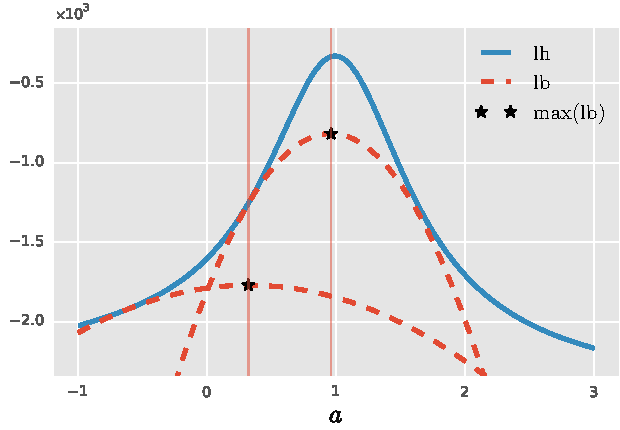
\includegraphics{img/ar1_ex_em}%
	\caption{%
Illustration of two iterations of the EM algorithm for a unidimensional parameter 
$\theta$. Starting from the lower left corner, given the current parameter estimate
$\theta_k$, the E-step computes the lower bound (dashed line) 
to the objective function $\lLH[\theta]$ (solid line). In the M-step, the next parameter 
value $\theta_{k+1}$ is found by maximizing the lower bound obtained in the E-step. The 
EM estimate is very close to the ML estimate at iteration $k+2$.
   	}
	\label{fig:ar1_em}
 \end{figure}

We have so far formulated the EM algorithm only for ML estimation. In the case
of MAP estimation with a nonuniform prior (remember that with a uniform prior the estimates are identical), 
the E-step stays the same since the prior is independent of $\X$.
The MAP M-step is
\begin{description}
\addtolength{\leftskip}{1cm}
  \item[M-step (MAP)]\hfill\\ 
  Set $\Th_{j+1}$ to the estimate that maximizes $\EMB{\gv{\psi}_{j+1}}{\Th}+\log\Pdf{\Th}$ with respect to $\Th$.
\end{description}%


 

%%%%%%%%%%%%%%%%%%%%%%%%%%%%%%%%%%%%%%%%%%%%%%%%%%%%%%%%%%%%%%%%%%%%%%%%%%%%%%%%%%
\subsubsection*{EM in exponential families of distributions}\label{sec:EM_exp}%
%%%%%%%%%%%%%%%%%%%%%%%%%%%%%%%%%%%%%%%%%%%%%%%%%%%%%%%%%%%%%%%%%%%%%%%%%%%%%%%%%%

Computing the intermediate quantity of EM is especially simple
if the dynamic model and the measurement model belong to an exponential
family of distributions, which have probability distribution functions of the form 
\begin{align}
	\Pdf[q]{\z}{\Th}&=\F{h}{\z}\exp\brac[\big]{ \F{\gv{\psi}}{\Th}^\tr \F*{s}{\z}-\F{c}{\Th}}.
	\label{eq:exp_family}
\end{align}
Here $\F*{s}{\z}$ is called the vector of \emph{natural sufficient statistics} and
$\gv{\eta}\equiv \F{\gv{\psi}}{\Th}$ is the \emph{natural parameterization}.
Let us suppose now that the complete-data likelihood is of the form \eqref{eq:exp_family}, so
that $\v{z}^\tr=\brak*{\mathrm{vec}\brac*{\X}^\tr,\mathrm{vec}\brac*{\Y}^\tr}$, where the operator $\mathrm{vec}\brac*{\cdot}$
creates vectors out of matrices by stacking their columns. Thus $\v{z}$ 
contains the hidden variables $\X$ and the measurements $\Y$. 

The intermediate quantity, which is the expectation of the logarithm of $\Pdf[q]{\z}{\Th}$ over the posterior
distribution of $\X$ (implicit in the notation) becomes now
\begin{align}
	\EMQ&=	\F{\gv{\psi}}{\Th}^\tr \E{\F*{s}{\z}}-\F{c}{\Th}+\E{\F{h}{\z}}.
\end{align}
Since the last term is independent of $\Th$ then the maximization in the M-step
is independent of this last term. Thus the role of the E-step degenerates into computing the
expectation of the sufficient statistics $\E{\F*{s}{\z}}$.



%%%%%%%%%%%%%%%%%%%%%%%%%%%%%%%%%%%%%%%%%%%%%%%%%%%%%%%%%%%%%%%%%%
\subsubsection*{EM as a special case of variational Bayes}%%%%%%
%%%%%%%%%%%%%%%%%%%%%%%%%%%%%%%%%%%%%%%%%%%%%%%%%%%%%%%%%%%%%%%%%%


Variational Bayes (VB) is a fully Bayesian methodology where one seeks
for an approximation to the parameter posterior \parencite{barber2012bayesian,Bishop2006,Mackay2004,beal2003variational}
\begin{align}
	\Pdf{\Th}{\Y} &= \frac{1}{Z}\Pdf{\Y}{\Th}\Pdf{\Th} \approx \Pdf[q]{\Th}. 
\end{align}
The appeal here is that when succesfull, fully Bayesian results can
be obtained with significantly reduced computational requirements
as compared to simulation based methods. Unfortunately it seems that applying
VB to SSMs is somewhat problematic, as discussed in \textcite{Turner2011}.   

Let us introduce the following simplifying
factorization to the joint posterior of states and parameters:
\begin{align}
	\Pdf{\X,\Th}{\Y}\approx \Pdf[q]{\X}\Pdf[q]{\Th}.
	\label{eq:VB_factorization}
\end{align}
Noting now that $\Pdf{\X,\Th}{\Y}=\Pdf{\X,\Y,\Th}/\LH$ and that $\lLH\equiv\log\LH$ is independent of $\X$ we can then perform the
following decomposition on the log likelihood:
\begin{align}
\begin{split}
	\lLH &= \log\Pdf{\X,\Y,\Th} - \log\Pdf{\X,\Th}{\Y} \\
	&= \E{\log\Pdf{\X,\Y,\Th}}_{\Pdf[q]{\X}\Pdf[q]{\Th}} - \E{\Pdf{\X,\Th}{\Y}}_{\Pdf[q]{\X}\Pdf[q]{\Th}} \\ 
	\begin{split}
	&=\E{\log\Pdf{\X,\Y,\Th}}_{\Pdf[q]{\X}\Pdf[q]{\Th}} -  \E{\Pdf[q]{\X}}_{\Pdf[q]{\X}} - \E{\Pdf[q]{\Th}}_{\Pdf[q]{\Th}}\\
	&\quad+\KL{\Pdf[q]{\X}\Pdf[q]{\Th}}{\Pdf{\X,\Th}{\Y}}. 
	\end{split}
\end{split}
	\label{eq:lLH_decomp_vb}
\end{align}
Thus minimizing the KL divergence between the factorized approximation and the true joint posterior is equivalent to finding the tightest lower bound to
the log likelihood. 
These considerations suggest an iterative algorithm
which produces a series of estimates $\Pdf[q_j]{\Th}$, where $j=0,\dots$.
Given the initial guess $\Pdf[q_0]{\Th}$, the two alternating
steps of the algorithm are:

\begin{description}
\addtolength{\leftskip}{1cm}
\item[E-step]
\begin{align}
	\Pdf[q_{j+1}]{\X}=\argmin_{\Pdf[q]{\X}}\KL{\Pdf[q]{\X}\Pdf[q_{j}]{\Th}}{\Pdf{\X,\Th}{\Y}}
	\label{eq:VB_E}
\end{align}
\item[M-step]
\begin{align}
	\Pdf[q_{j+1}]{\Th}=\argmin_{\Pdf[q]{\Th}}\KL{\Pdf[q_{j+1}]{\X}\Pdf[q]{\Th}}{\Pdf{\X,\Th}{\Y}}
	\label{eq:VB_M}
\end{align}
\end{description}

Let us then suppose that we only wish to find the MAP estimate $\Th^*$. This can be accomplished
by assuming a delta function form $\Pdf[q]{\Th}=\delta\left(\Th,\Th^*\right)$ for the parameter factor in the
joint distribution of states and parameters \eqref{eq:VB_factorization}.
With this assumption the bound becomes
\begin{align}
	\Pdf{\Y}{\Th^*} &\geq \E{\log\Pdf{\X,\Y,\Th}}_{\Pdf[q]{\X}\Pdf[q]{\Th^*}} -  \E{\Pdf[q]{\X}}_{\Pdf[q]{\X}} +
	\mathtt{const}
	\label{eq:VB_MAP_boundl}
\end{align}
and the ``M''-step \eqref{eq:VB_M} can then be written as
\begin{align}
	\Th_{j+1} &= \argmax_{\Th}\brak*{\E{\log\cLH}_{\Pdf[q]{\X}}+\log\Pdf{\Th}}.	
\end{align}
If the point estimate is plugged in the ``E''-step Equation~\eqref{eq:VB_E} we get
\begin{align}
	\Pdf[q_{j+1}]{\X}\propto \Pdf{\X,\Y}{\Th_j} \propto \Pdf{\X}{\Y,\Th_j}.
\end{align}
Thus the EM algorithm can shown to be a special case of VB with a delta function form
for $\Pdf[q]{\Th}$.


%%%%%%%%%%%%%%%%%%%%%%%%%%%%%%%%%%%%%%%%%%%%%%%%%
\subsubsection{Partial E and M steps}%%%%%%%%%%
%%%%%%%%%%%%%%%%%%%%%%%%%%%%%%%%%%%%%%%%%%%%%%%%%
\label{sec:EM_partial}
As can be seen from Equation~\eqref{eq:fundamental_inequality},
to ensure monotonicity it is enough that $\EMQ{\Th_j}{\Th_{j+1}}\geq \EMQ{\Th_{j}}{\Th_j}$,
which means $\Th_{j+1}$ is not required to be the maximum of $\EMQ{\Th_j}{\Th}$.
This was observed already in \textcite{Dempster1977}, where methods
that only seek an increase in the M-step were termed 
\emph{generalized} EM (gEM) algorithms. 

Another modification is the partial, or approximate, E-step. It is clear
that in this case, when we cannot compute $\post$ exactly, the Kullback-Leibler 
divergence in decomposition \eqref{eq:lLH_decomp} is strictly positive. This
means that the lower bound we are optimizing never ``touches'' the log-likelihood
as in Equation~\eqref{eq:EM_sharp_bound} and Figure~\ref{fig:ar1_em}. 
Thus EM with an approximate  E step is not an ascent 
algorithm anymore \parencite{Goodwin2005}.

% When we restrict the approximation $\tPX$ to $\post$ to a certain
% family of probability distribution and choose the one which
% minimizes $\KL{\tPX}{\post}$, the resulting algorithm is known
% as \emph{variational Expectation Maximization} (vEM) \parencite{Turner2011}.
% When we restrict $\tPX$ to be Gaussian via moment matching, as is the case
% in Gaussian filtering/smoothing, this KL divergence is in fact minimized.
% Suppose now that $\gv{\psi}\equiv \brac{\m,\P}$, where $\m$ is the mean and \todo{fill up the moment matching KL equations}
% $\P$ is the covariance matrix. Then
% \begin{align}
% 	\dpd{}{\m}\KL{\tPX}{\post} &= \\
% 	\dpd{}{\P}\KL{\tPX}{\post} &=.
% \end{align}
% Setting these simultaneously to zero we obtain
% \begin{align}
% 	\dpd{\KL{\tPX}{\post}}{\m} &= \\
% 	\dpd{\KL{\tPX}{\post}}{\P} &=
% \end{align}


%%%%%%%%%%%%%%%%%%%%%%%%%%%%%%%%%%%%%%%%%%%%%%%%
\subsubsection{Linear-Gaussian SSMs}%%%%%%%%%%
%%%%%%%%%%%%%%%%%%%%%%%%%%%%%%%%%%%%%%%%%%%%%%%%
\label{sec:EM_SSM}

Let us then turn to applying EM to the case of linear-Gaussian SSMs
\parencite{shumway1982approach,Ghahramani1996}
, so that
\begin{align*}
	\ff &\equiv \v{A}\xkk\\
	\hh &\equiv \v{H}\xk\\
	\Th &\equiv \brac{\v{A},\v{Q},\v{H},\v{R}}.
\end{align*}
First of all, from the factorization in \eqref{eq:complete_data_likelihood}, the complete-data log-likelihood becomes
\begin{align}
\begin{split}
	\lLH
	=&-\frac{1}{2}\left(\x_0-\gv{\mu}_0\right)^\tr\gv{\Sigma}_0^{-1}\left(\x_0-\gv{\mu}_0\right)-\frac{1}{2}\log\detr{\gv{\Sigma}_0}\\
	&-\frac{1}{2}\sum_{k=1}^T\left(\x_k-\v{A}\xkk\right)^\tr\v{Q}^{-1}\left(\x_k-\v{A}\xkk\right)-\frac{T}{2}\log\detr{\v{Q}}\\
	&-\frac{1}{2}\sum_{k=1}^T\left(\y_k-\v{H}\xk\right)^\tr\v{R}^{-1}\left(\y_k-\v{H}\xk\right)-\frac{T}{2}\log\detr{\v{R}}\\
	&+\mathtt{const}.
\end{split}
\label{eq:clLH_LG}
\end{align}
Taking the expectation of \eqref{eq:clLH_LG} with respect to $\Pdf{\X}{\Y,\Th'}$ (assumed implicitly in the notation),
applying the identity $\v{a}^\tr\v{C}\v{b}=\Tr{\v{a}^\tr\v{C}\v{b}}=\Tr{\v{C}\v{b}\v{a}^\tr}$, and dropping the constant terms we get
\begin{align}
\begin{split}
	\EMQ{\Th'}{\Th} \approx -\frac{1}{2}\bigg\{&\Tr{\gv{\Sigma}_0^{-1}\E{\left(\x_0-\gv{\mu}_0\right)\left(\x_0-\gv{\mu}_0\right)^\tr}}+\log\detr{\gv{\Sigma}_0}\\
	+\,&\Tr[\bigg]{\v{Q}^{-1}\sum_{k=1}^T\E{\left(\x_k-\v{A}\xkk\right)\left(\x_k-\v{A}\xkk\right)^\tr}}+T\log\detr{\v{Q}}\\
	+\,&\Tr[\bigg]{\v{R}^{-1}\sum_{k=1}^T\E{\left(\y_k-\v{H}\xk\right)\left(\y_k-\v{H}\xk\right)^\tr}}+T\log\detr{\v{R}}\bigg\}.
\end{split}
\label{eq:eclLH}
\end{align} 
Let us denote the quadratic forms inside the traces in Equation~\eqref{eq:eclLH} with
\begin{align}
	\begin{split}
	\II{1} &= 
	\E{\left(\x_0-\gv{\mu}_0\right)\left(\x_0-\gv{\mu}_0\right)^\tr}\\ 
	&=\defint{\mathcal{X}\times T}{}{\left(\x_0-\gv{\mu}_0\right)\left(\x_0-\gv{\mu}_0\right)^\tr\Pdf{\X}{\Y,\Th'}}{\X}\\
	&= 	\defint{\mathcal{X}}{}{\left(\x_0-\gv{\mu}_0\right)\left(\x_0-\gv{\mu}_0\right)^\tr\Pdf{\x_0}{\Y,\Th'}}{\x_0} 
	\end{split}\label{eq:I1_general}\\
%
	\begin{split}
	\II{2} &= \sum_{k=1}^T\defint{\mathcal{X}}{}{\left(\x_k-\v{A}\xkk\right)\left(\x_k-\v{A}\xkk\right)^\tr\\
	& \qquad \times\Pdf{\xk,\xkk}{\Y,\Th'}}{\xk}{\xkk}
	\end{split}\label{eq:I2_general}\\
%	
	\begin{split}
	\II{3}& =
	\sum_{k=1}^T\defint{\mathcal{X}}{}{\left(\y_k-\v{H}\xk\right)\left(\y_k-\v{H}\xk\right)^\tr\Pdf{\xk}{\Y,\Th'}}{\xk}
	\end{split}.\label{eq:I3_general}
\end{align}
%
It is clear then that in the E-step one needs to compute the $T+1$ smoothing
distributions, including the $T$ cross-timestep distributions, since these
will be needed in the expectations.
By applying the identity
\begin{align}
	\var{\x}&=\E{\x\x^\tr}-\E{\x}\E{\x}^\tr,
\end{align} 
we can write the first expectation as
\begin{align}
	\II{1}&= \v{P}_{0|T}+(\v{m}_{0|T}-\gv{\mu}_0)(\v{m}_{0|T}-\gv{\mu}_0)^\tr.
	\label{eq:I1}
\end{align}
%where we denote Gaussian smoothing distributions by $\Pdf{\xk}{\Y}=\N[\xk]{\m_{k|T}}{\P_{k|T}}$.
This was a result of assuming the Gaussian prior distribution of Equation~\eqref{eq:prior}.

As in \eqref{eq:joint_smoothing}, let us denote the joint smoothing distribution of $\xk$ and $\xkk$ by
\begin{align}
\Pdf{\xkk,\xk}{\Y}&=\N[\bm{\xkk\\\xk}]{
	\bm{
		\m_{k-1|T}\\
		\m_{k|T}
	}}{
	\bm{
		\P_{k-1|T}&\v{D}_{k-1}\\
		\v{D}_{k-1}^\tr&\P_{k|T}
	}}
	\label{eq:pdf_smooth_joint}.
\end{align}
Then by applying the manipulation
\begin{align}
\begin{split}
&\E{\left(\v{A}\v{x}_{k-1}-\v{x}_k\right)\left(\v{A}\v{x}_{k-1}-\v{x}_k\right)^\tr}\\
=&\bm{\v{A}^\tr \\ -\v{I}}^\tr	
\E{
\begin{bmatrix}
	\xkk\\\xk
\end{bmatrix}
\begin{bmatrix}
	\xkk \\ \xk	
\end{bmatrix}^\tr
}
\bm{\v{A}^\tr\\-\v{I}}	
\end{split}
\end{align}
we get
\begin{align}
	\II{2}&=
\bm{\v{A}^\tr \\ -\v{I}}^\tr	
\sum_{k=1}^T\left(\bm{
		\P_{k-1|T}&\v{D}_{k-1}\\
		\v{D}_{k-1}^\tr&\P_{k|T}
	}+\bm{
		\m_{k-1|T}\\
		\m_{k|T}
	}\bm{
		\m_{k-1|T}\\
		\m_{k|T}
	}^\tr\right)
\bm{\v{A}^\tr\\-\v{I}}	\label{eq:LGSSM_I2}\\
&=%
%
\bm{\v{A}^\tr \\ -\v{I}}^\tr	
%\bm{\P_{k|T}+\m_{k|T}\m_{k|T}^\tr & \left(\P_{k,k-1|T}+\m_{k,k-1|T}\m_{k,k-1|T}^\tr\right)^\tr \\ \P_{k,k-1|T}+\m_{k,k-1|T}\m_{k,k-1|T}^\tr & \P_{k-1|T}+\m_{k-1|T}\m_{k-1|T}^\tr }
\bm{\sum_{k=1}^T\E{\xkk\xkk^\tr} & \sum_{k=1}^T\E{\xkk\xk^\tr} \\ \sum_{k=1}^T\E{\xk\xkk^\tr} &
\sum_{k=1}^T\E{\xk\xk^\tr} } \bm{\v{A}^\tr\\-\v{I}}	\nonumber\\
%
&=%
\bm{\v{A}^\tr \\ -\v{I}}^\tr	
\bm{\XX_{11} & \XX_{10} \\ \XX_{10}^\tr & \XX_{00} }
\bm{\v{A}^\tr\\-\v{I}}	\nonumber\\
%
&=\XX_{00}-\v{A}\XX_{10}-\XX_{10}^\tr\v{A}^\tr+\v{A}\XX_{11}\v{A}^\tr\nonumber\\
&=\left(\v{A}-\XX_{10}^\tr\XX_{11}^{-1}\right)\XX_{11}\left(\v{A}-\XX_{10}^\tr\XX_{11}^{-1}\right)^\tr+\XX_{00}+\XX_{10}^\tr\XX_{11}^{-1}\XX_{10}.
\label{eq:Amax}
\end{align}
It's easy to see that the extremum of the last line with respect to $\v{A}$
is obtained by setting
\begin{align}
	\v{A}_{j+1}&=\XX_{10}^\tr\XX_{11}^{-1} \label{eq:EM_M_A}.	
\end{align}
Analogously for $\II{3}$ we get
\begin{align}
\II{3}&=
\bm{\v{I} \\ -\v{H}^\tr}^\tr	
\sum_{k=1}^T
\bm{\yk\yk^\tr & \yk\E{\xk}^\tr \\ \E{\xk}\yk^\tr & \E{\xk\xk^\tr} }
\bm{\v{I}\\-\v{H}^\tr} \label{eq:LGSSM_I3}\\
&=\bm{\v{I} \\ -\v{H}^\tr}^\tr	
\sum_{k=1}^T
	\bm{\YY_{00} & \bar{\v{C}}_{00} \\ \bar{\v{C}}_{00}^\tr & \XX_{00} }
\bm{\v{I}\\-\v{H}^\tr},
\end{align}
giving
\begin{align}
	\v{H}_{j+1}&=\bar{\v{C}}_{00}\XX_{00}^{-1} \label{eq:EM_M_H}.	
\end{align}


The next task is to derive the M-step maximization equations for the 
process and measurement model noise covariance matrices $\v{Q}$ and $\v{R}$. 
To achieve this, we will differentiate \eqref{eq:eclLH} with respect to
these matrices. As can be seen from \eqref{eq:eclLH}, the terms involving $\v{Q}$ or $\v{R}$
are similar in form and so the resulting maximization equations are analogous.
Focusing on $\v{Q}$, it is easier to differentiate with respect to $\v{Q}^{-1}$:
\begin{align}
	\dpd{\EMQ{\Th'}{\Th}}{\v{Q^{-1}}}=
	&-\frac{1}{2}\dpd{}{\v{Q^{-1}}}\Tr[\bigg]{\v{Q}^{-1}\sum_{k=1}^T\E{\left(\xk-\f_{k-1}\right)\left(\xk-\f_{k-1}\right)^\tr}}\nonumber\\
	&-\frac{T}{2}\dpd{}{\v{Q^{-1}}}\log\det{\v{Q}}\nonumber\\
	=&-\frac{1}{2}\sum_{k=1}^T\E{\left(\xk-\f_{k-1})\right)\left(\xk-\f_{k-1})\right)^\tr}+\frac{T}{2}\v{Q},
	\label{eq:clLH_pdQ}
\end{align}
where we have used Equations (92) and (51) in \cite{Petersen2008}. Setting \eqref{eq:clLH_pdQ}  
to zero \todo{Why is it same for the inverse?} we get the update equation for the next estimate of $\v{Q}$
\begin{align}
\begin{split}
	\v{Q}_{j+1}&=\frac{1}{T}\sum_{k=1}^T\E{\left(\xk-\f_{k-1}\right)\left(\xk-\f_{k-1}\right)^\tr} \label{eq:EM_M_Q}\\
	&=\frac{1}{T}\II{2}.
\end{split}
\end{align}
The analogous result for $\v{R}$ is given by
\begin{align}
\begin{split}
	\v{R}_{j+1}&=\frac{1}{T}\sum_{k=1}^T\E{\left(\yk-\h_{k}\right)\left(\yk-\h_{k}\right)^\tr} \label{eq:EM_M_R}\\
	&=\frac{1}{T}\II{3}.
	\end{split}
\end{align} 

All in all, the E-step of the EM algorithm in linear-Gaussian SSMs consists of
computing the $T$ joint distributions of Equation~\eqref{eq:pdf_smooth_joint} with the RTS smoother.
%Actually this is not the only option, as for example in
%\textcite{Elliott1999} a new kind of filter is presented that
%can compute the expectations with only forward recursions.
After this, the M-step estimates are computed for $\v{Q}$
from Equation~\eqref{eq:EM_M_Q}, for $\v{R}$ from Equation~\eqref{eq:EM_M_R}, for $\v{A}$ from
Equation~\eqref{eq:EM_M_A} and for $\v{H}$ from Equation~\eqref{eq:EM_M_H}. 

%Also for evaluating the convergence,
%one needs to compare the current value of $\EMQ$ with the previous one.
%For this we can compute $\II{1}$ from Equation~\eqref{eq:I1},
%$\II{2}$ from Equation~\eqref{eq:LGSSM_I2} and $\II{3}$ from Equation~\eqref{eq:LGSSM_I3}.

% For working with structured matrices let us rewrite the gradient equation~\eqref{eq:dLB_nonlinear}
% in the linear-Gaussian case:
% 
% \begin{align}
% \label{eq:dLB_linear}
% \begin{split}
% 	\dpd{\EMQ{\Th}{\Th'}}{\theta_i}
% 	=\quad{}&\frac{1}{2}\mathrm{Tr}\!\Bigg[\gv{\Sigma}^{-1}\bigg(
% 	\dpd{\gv{\Sigma}}{\theta_i}\gv{\Sigma}^{-1}
% 	\sum_{k=1}^T\E{\left(\x_0-\gv{\mu}_0\right)\left(\x_0-\gv{\mu}_0\right)^\tr}{\hat{\Th}_j}\\
% 	&\quad+2\sum_{k=1}^T\E[\Big]{\dpd{\gv{\mu}_0}{\theta_i}\left(\x_0-\gv{\mu}_0\right)^\tr}
% 	-\dpd{\gv{\Sigma}}{\theta_i}\bigg)\Bigg]\\
% %
% 	+&\frac{1}{2}\mathrm{Tr}\!\Bigg[\v{Q}^{-1}\bigg(\dpd{\v{Q}}{\theta_i}\v{Q}^{-1}
% 	\bm{\v{I} & -\v{A}}\bm{\XX_{00} & \XX_{01} \\ \XX_{01}^\tr & \XX_{11} }\bm{\v{I}\\-\v{A}^\tr}\\	
% 	&\quad +2\bm{\v{0} & -\dpd{\v{A}}{\theta_i}}\bm{\XX_{00} & \XX_{01} \\ \XX_{01}^\tr & \XX_{11} }\bm{\v{I}\\-\v{A}^\tr}
% 	-T\dpd{\v{Q}}{\theta_i}\bigg)\Bigg]\\
% %	
% 	+&\frac{1}{2}\mathrm{Tr}\!\Bigg[\v{R}^{-1}\bigg(\dpd{\v{R}}{\theta_i}\v{R}^{-1}
% 	\bm{\v{I} & -\v{H}}\bm{\YY_{00} & \bar{\v{C}}_{00} \\ \bar{\v{C}}_{00}^\tr & \XX_{00} }\bm{\v{I}\\-\v{H}^\tr}\\
% 	&\quad +2\bm{\v{0} & -\dpd{\v{H}}{\theta_i}}\bm{\YY_{00} & \bar{\v{C}}_{00} \\ \bar{\v{C}}_{00}^\tr & \XX_{00} }\bm{\v{I}\\-\v{H}^\tr}
% 	-T\dpd{\v{R}}{\theta_i}\bigg)\Bigg].
% \end{split}	
% \end{align}

%%%%%%%%%%%%%%%%%%%%%%%%%%%%%%%%%%%%%%%%%%%%%%%%%%%%%%%%%%%%%%%%%%%%%%%%%%
\subsubsection{Nonlinear-Gaussian SSMs} \label{sec:EM_nonlinear}%%%%%%%%%%
%%%%%%%%%%%%%%%%%%%%%%%%%%%%%%%%%%%%%%%%%%%%%%%%%%%%%%%%%%%%%%%%%%%%%%%%%%

As explained in Section~\ref{sec:nonlinear_state}, in the nonlinear case
the filtering and smoothing distributions cannot be computed exactly.
Thus the E-step is approximate and the convergence
guarantees of EM as an ascent method won't apply anymore. In the fortunate case that the
model is linear-in-the-parameters the M-step can be solved in closed form.
This situation will be covered later in Section~\ref{sec:litp}. 
Currently we will assume however that the model is nonlinear in the 
parameters as well as in the states so that the simplest form to write the 
model is given by Equation~\eqref{eq:ssm_general}. This situation leads to 
complications in both the E and the M steps of the EM algorithm.
Applying EM to SSMs with partial or approximate E-step is considered
at least in \textcite{Schon2011,Ratna2008,Doucet2001,Roweis2001},  and \textcite{Goodwin2005}.

Our strategy will be to apply Gaussian filtering and smoothing
in the E-step to compute the expectations of the sufficient statistics.
We will settle for an incremental M-step where we again apply a gradient based optimization method.
This leads to the requirement of being able to compute 
$\nabla_{\Th}\EMQ$, that is the gradient of the intermediate quantity with respect
to $\Th$. It is quite unclear how many iterations of the optimization algorithm should
be run in the M-step since, as pointed out in section~\ref{sec:EM_partial},
\emph{any} new parameter value that increases the log-likehood suffices. In \textcite{Lange1995}
a heuristic argument was used to only run a single iteration of Newton's method in the M-step.

Denoting $\f_{k-1}\equiv \ff$ and $\h_k\equiv \hh$, we now have
\begin{align}
\label{eq:EMQ_approx}
\begin{split}
	\EMQ{\Th'}{\Th} \approx -\frac{1}{2}\bigg\{&\Tr{\gv{\Sigma}_0^{-1}\II{1}}+\log\detr{\gv{\Sigma}_0}\\
	+\,&\Tr[\Big]{\v{Q}^{-1}\III{2}}+T\log\detr{\v{Q}}\\
	+\,&\Tr[\Big]{\v{R}^{-1}\III{3}}+T\log\detr{\v{R}}\bigg\},
\end{split}
\end{align}
where $\II{1}$ was given in Equation~\eqref{eq:I1_general} and
we approximate
\begin{align}
	\Pdf{\xk,\xkk}{\Y,\Th'}&\approx \N[\bm{\xkk\\\xk}]{
	\begin{bmatrix}
		\m_{k-1|T}\\
		\m_{k|T}
	\end{bmatrix}}{
	\begin{bmatrix}
		\P_{k-1|T}&\v{D}_{k-1}\\
		\v{D}_{k-1}^\tr&\P_{k|T}
	\end{bmatrix}
	}
	\label{eq:smooth_approx}
\end{align}
giving
\begin{align}
\begin{split}
\III{2} &= \sum_{k=1}^T\iint_\mathcal{X}\left(\x_k-\ff\right)\left(\x_k-\ff\right)^\tr\\
&\quad \times \N[\bm{\xkk\\\xk}]{
	\begin{bmatrix}
		\m_{k-1|T}\\
		\m_{k|T}
	\end{bmatrix}}{
	\begin{bmatrix}
		\P_{k-1|T}&\v{D}_{k-1}\\
		\v{D}_{k-1}^\tr&\P_{k|T}
	\end{bmatrix}
	}
	\,\dif\xkk\dif\xk \\
&=
\bm{\v{I} \\ -\v{I}}^\tr	
\sum_{k=1}^T
\E{\bm{\xk \\ \f_{k-1}}\bm{\xk \\ \f_{k-1}}^\tr} 
\bm{\v{I}\\-\v{I}}
\end{split}\label{eq:I2_approx}\\	
\shortintertext{and}
\begin{split}
\III{3} &=
\sum_{k=1}^T\defint{\mathcal{X}}{}{\left(\y_k-\hh\right)\left(\y_k-\hh\right)^\tr\N[\xk]{\m_{k|T}}{\P_{k|T}}}{\xk} \\
&=
\bm{\v{I} \\ -\v{I}}^\tr	
\sum_{k=1}^T
\E{\bm{\yk \\ \h_{k}}\bm{\yk \\ \h_{k}}^\tr} 
\bm{\v{I}\\-\v{I}}.
\end{split}\label{eq:I3_approx}	
\end{align}
Clearly the integrals \eqref{eq:I2_approx} and \eqref{eq:I3_approx} are Gaussian
expectation integrals of the form \eqref{eq:gauss_integral}. An obvious
strategy is thus to utilize a Gaussian smoother to compute the joint
smoothing distributions and then compute the $2T$ expectation integrals
by applying the same integration rule as was used by the smoother. 

To use gradient based nonlinear optimization in the M-step, we will need the analytical gradient of the objective
function. It is important to highlight at this point that the joint smoothing distribution approximation
of Equation~\eqref{eq:smooth_approx} depends on $\Th'$ (the \emph{current}, e.g. given, parameter value)
and during the M-step we are searching for the \emph{next} parameter value $\Th^{\prime\prime}=\argmax_{\Th}\EMQ$. In
other words when differentiating the integrals \eqref{eq:I2_approx} and \eqref{eq:I3_approx} the Gaussian functions
are independent of $\Th$.
Let us then find out the formal differential of a general log-Gaussian, where
both the mean and the variance depend on the scalar parameter $\theta$. We get
\begin{align*}
\begin{split}
	\dpd{}{\theta}&\log\N[\x]{\m}{\P}\\
	&=-\frac{1}{2}\dpd{}{\theta}\brak*{(\x-\m)^\tr\P^{-1}(\x-\m)}-\frac{1}{2}\dpd{}{\theta}\log\detr\P\\		
	&=-\frac{1}{2}\dpd{}{\theta}\Tr{\P^{-1}(\x-\m)(\x-\m)^\tr}-\frac{1}{2}\Tr{\P^{-1}\dpd{\P}{\theta}}\\		
	&=\frac{1}{2}\Tr{\P^{-1}\fparen*{\dpd{\P}{\theta}\P^{-1}(\x-\m)(\x-\m)^\tr+2\dpd{\m}{\theta}(\x-\m)^\tr-\dpd{\P}{\theta}}}		
\end{split}
	%&= \fparen*{\fparen*{2\pi}^{d_x}\detr\P}^{-\sfrac{1}{2}}\exp\fparen*{-\frac{1}{2}
	%\Tr{\P^{-1}\bm{\v{I}\\-\v{I}}^\tr\bm{\x\\\m}\bm{\x\\\m}^\tr\bm{\v{I}\\-\v{I}}}},		
\end{align*}


If we then assume
that $\ff$ , $\v{Q}$, $\hh$, $\v{R}$, $\gv{\mu}_0$ and $\gv{\Sigma}_0$ depend on $\theta_i\in\Th$,
we can write
\begin{align}
	\nabla_{\Th}\EMQ &= \bm{\dpd{\EMQ}{\theta_1}&\dots&\dpd{\EMQ}{\theta_{d_\theta}}}^\tr
\end{align}
and
\begin{align}
\label{eq:dLB_nonlinear}
\begin{split}
	\dpd{\EMQ}{\theta_i}&\approx\\
%	
	&\frac{1}{2}\mathrm{Tr}\!\bigg[\gv{\Sigma}_0^{-1}\bigg(
	\dpd{\gv{\Sigma}_0}{\theta_i}\gv{\Sigma}_0^{-1}
	\II{1}
	+2\dpd{\gv{\mu}_0}{\theta_i}\left(\m_{0|T}-\gv{\mu}_0\right)^\tr
	-\dpd{\gv{\Sigma}_0}{\theta_i}\bigg)\bigg]\\
%	
	+&\frac{1}{2}\mathrm{Tr}\!\bigg[\v{Q}^{-1}\bigg(\dpd{\v{Q}}{\theta_i}\v{Q}^{-1}
	\III{2}
	+2\sum_{k=1}^T\E[\Big]{\dpd{\ff}{\theta_i}\x_k^\tr}\\%
	&\qquad-2\sum_{k=1}^T\E[\Big]{\dpd{\ff}{\theta_i}\ff^\tr}
	-T\dpd{\v{Q}}{\theta_i}\bigg)\bigg]\\
%	
	+&\frac{1}{2}\mathrm{Tr}\!\bigg[\v{R}^{-1}\bigg(\dpd{\v{R}}{\theta_i}\v{R}^{-1}
	\III{3}
	+2\sum_{k=1}^T\E[\Big]{\dpd{\hh}{\theta_i}}\y_k^\tr\\
	&\qquad-2\sum_{k=1}^T\E[\Big]{\dpd{\hh}{\theta_i}\hh^\tr}
	-T\dpd{\v{R}}{\theta_i}\bigg)\bigg].
\end{split}	
\end{align}
In order to gather the computations needed evaluate $\EMQ$ and $\nabla_{\Th}\EMQ$ given the sufficient statistics
of the $T$ joint smoothing distributions, let us introduce the shorthand notation 
$\f^{\nabla}_{k-1,i}\equiv\dpd{\ff}{\theta_i}$
and  $\h^\nabla_{k,i}\equiv\dpd{\hh}{\theta_i}$.
One should then
perform the following operations:
\begin{enumerate}
  \item For $k=1,\dots,T$ and $i=1,\dots,d_\theta$, apply a numerical integration scheme to compute
%  
\begin{align}
\E{\bm{\xk \\ \f_{k-1} \\ \f^\nabla_{k-1,i}}\bm{\xk \\ \f_{k-1} \\ \f^\nabla_{k-1,i}}^\tr} 		
\end{align}
and
\begin{align}
\E{\bm{\yk \\ \h_{k} \\ \h^\nabla_{k,i}}\bm{\yk \\ \h_{k} \\ \h^\nabla_{k,i}}^\tr}.		
\end{align}
\item Compute $\II{1}$, $\III{2}$, $\III{3}$ and $\EMQ$ from Equations
\eqref{eq:I1}, \eqref{eq:I2_approx}, \eqref{eq:I3_approx} and \eqref{eq:EMQ_approx} respectively.
\item Compute $\nabla_{\Th}\EMQ$ from Equation \eqref{eq:dLB_nonlinear}.
\end{enumerate}


%%%%%%%%%%%%%%%%%%%%%%%%%%%%%%%%%%%%%
\subsubsection{Score computation}\label{sec:fisheri}%%
%%%%%%%%%%%%%%%%%%%%%%%%%%%%%%%%%%%%%

As can be understood from Fisher's identity in Equation~\eqref{eq:EM_gradients},
the gradient of the intermediate quantity $\nabla_{\Th}\EMQ$ is equal to the log-likelihood
gradient (the score) at the point $\Th=\Th'$. This leads to an alternative computational
strategy to the sensitivity equations of Section~\ref{sec:grad_LGSSM}, termed
the \emph{easy gradient recipe} in \textcite{Olsson2007}. Thus to compute the score
at $\Th'$ one performs the computations detailed in the previous section for evaluating
$\nabla_{\Th}\EMQ{\Th'}{\Th'}$. 
Using gradient based
optimization for $\lLH$, where
$\score$ is computed through the Fisher's identity 
is also the idea in the expectation-conjugate-gradient (ECG) method of \textcite{Salakhutdinov2003a}. 


%%%%%%%%%%%%%%%%%%%%%%%%%%%%%%%%%%%%%%%%%%%%%%%%%%%%%%%%%
\subsubsection*{Linear-in-the-parameters SSM:s}%%%%%
%%%%%%%%%%%%%%%%%%%%%%%%%%%%%%%%%%%%%%%%%%%%%%%%%%%%%%%%%
\label{sec:litp}

If the dynamic and measurement models are linear-in-the-parameters but nonlinear
in the states, then only the E-step is approximate and the M-step can be performed
in closed form. Thus this situation is a combination of the linear-Gaussian
and the nonlinear-Gaussian cases discussed in the previous sections.

Suppose now that $\f:\mathcal{X}\to\mathcal{X}$ is a linear
combination of vector valued functions $\gv{\rho}_j:\mathcal{X}\to\R^{d_{\Phi,j}}$,
so that the parameters of $\f$, $\gv{\Phi}_j$, are matrices of size $d_x\times d_{\Phi,j}$.
Then $\f$ can be written as 
\begin{align}
\begin{split}
	\ff &=\gv{\Phi}_1(\Th)\gv{\rho}_1(\xkk)+\dots+\gv{\Phi}(\Th)_m\gv{\rho}_m(\xkk)\\
	&=
	\begin{bmatrix}
		\gv{\Phi}(\Th)_1 & \dots & \gv{\Phi}(\Th)_m
	\end{bmatrix}
	\begin{bmatrix}
		\gv{\rho}_1(\xkk)\\
		\vdots\\ 
		\gv{\rho}_m(\xkk)
	\end{bmatrix}\\
	&=\v{A}(\Th)\v{g}(\xkk),
\end{split}
\end{align}
so that $\v{A}(\Th)$ is now a matrix of size ${d_x\times\sum_{j=1}^m d_{\Phi,j}}$ and $\v{g}:\mathcal{X}\to
\R^{\sum_{j=1}^m d_{\Phi,j}}$ .
Denoting $\v{g}\left(\xkk\right)\equiv\v{g}_{k-1}$ 
and following the derivation in Equation~\eqref{eq:LGSSM_I2} we now have
\begin{align}
	\III{2}
	&=\bm{\v{I} \\ -\v{A}^\tr}^\tr	
	\bm{\sum_{k=1}^T\E{\xk\xk^\tr} & \sum_{k=1}^T\E{\xk\v{g}_{k-1}^\tr} \\ 
		\sum_{k=1}^T\E{\v{g}_{k-1}\xk^\tr} & \sum_{k=1}^T\E{\v{g}_{k-1}\v{g}_{k-1}^\tr} }
	\bm{\v{I}\\-\v{A}^\tr}
	%&=\bm{\v{I} & -\v{A}}	
	%\bm{\bar{\X}_{00} & \bar{\v{G}}_{01} \\ \bar{\v{G}}_{01}^\tr & \bar{\v{G}}_{11} }
	%\bm{\v{I}\\-\v{A}^\tr}
\label{eq:I2_LIP}
\end{align}
Then similarly to \eqref{eq:EM_M_A}
\begin{align}
	\v{A}_{j+1}&=\fparen[\Big]{\sum_{k=1}^T\E{\xk\v{g}_{k-1}^\tr}}\fparen[\Big]{\sum_{k=1}^T\E{\v{g}_{k-1}\v{g}_{k-1}^\tr}}^{-1}.	
\end{align}
%
Analogously for $\h$ we can write
\begin{align}
\begin{split}
	\hh&=\gv{\Upsilon}_1(\Th)\gv{\pi}_1(\xk)+\dots+\gv{\Upsilon}_m(\Th)\gv{\pi}_m(\xk)\\
	&=
	\begin{bmatrix}
		\gv{\Upsilon}_1 & \dots & \gv{\Upsilon}_m
	\end{bmatrix}
	\begin{bmatrix}
		\gv{\pi}_1(\xk)\\
		\vdots\\ 
		\gv{\pi}_m(\xk)
	\end{bmatrix}\\
	&=\v{H}(\Th)\v{b}(\xk),
\end{split}
\end{align}
where $\v{H}(\Th)$ is now ${d_x\times\sum_{j=1}^m d_{\Upsilon,j}}$ and 
$\v{b}:\mathcal{X}\to \R^{\sum_{j=1}^m d_{\Upsilon,j}}$ .
Denoting $\v{b}\left(\xk\right)\equiv\v{b}_{k}$, we get
\begin{align}
	\III{3}&=
	\bm{\v{I} \\ -\v{H}^\tr}^\tr	
	\sum_{k=1}^T
	\bm{\yk\yk^\tr 		   & \yk\E{\v{b}_k}^\tr \\ 
		\E{\v{b}_k}\yk^\tr & \E{\v{b}_k\v{b}_k^\tr} }
	\bm{\v{I}\\-\v{H}^\tr} \label{eq:I3_LIP},
%	&=\bm{\v{I} & -\v{H}}	
	%\sum_{k=1}^T
%		\bm{\bar{\Y}_{00} & \bar{\v{D}}_{00} \\ \bar{\v{D}}_{00}^\tr & \bar{\v{L}}_{00} }
	%\bm{\v{I}\\-\v{H}^\tr} \nonumber,
\end{align}
giving
\begin{align}
	\v{H}_{j+1}&=\fparen[\Big]{\yk\E{\v{b}_k}^\tr}\fparen[\Big]{\E{\v{b}_k\v{b}_k^\tr}}^{-1} \label{eq:EM_LIP_M_H}.	
\end{align}


% %%%%%%%%%%%%%%%%%%%%%%%%%%%%%%%%%%%%%%%%%%%%%
% \subsection{Theoretical considerations}\label{sec:theory}%%%%%%
% %%%%%%%%%%%%%%%%%%%%%%%%%%%%%%%%%%%%%%%%%%%%%
% \subsubsection{Ascent methods}

An important theoretical result concerning iterative ascent methods is known
as the \emph{global convergence theorem} \parencite{luenberger2008}. It states
the necessary conditions that the estimate produced by an iterative ascent method
is a local maximum. Suppose then that $\ell:\Theta\to\R$ is the objective function
and we are trying to solve the \emph{unconstrained} optimization problem
\begin{align}
	\Th_\star&=\argmax_{\Th}\lLH,\quad\Th\in\Theta=\R^{d_\theta},
	\label{eq:optimization_problem}
\end{align}
where $\Th_\star$ need not be unique, i.e. there can be a solution set 
\begin{align}
	\mathcal{S}=\brac*{\Th_\star\in\Theta : \lLH[\Th_\star]\geq \lLH[\Th] \; \forall \Th\in\Theta}
\end{align}
To formulate the conditions under which this problem can be solved by an iterative ascent method,
we need to define the concept of a closed point-to-set mapping. $T$ is a point-to-set map
from $X$ to $Y$, if it maps points in $X$ to subsets of $Y$.
$T$ is said to be \emph{closed} at $\x \in X$ if
\begin{alignat*}{3}
	\mathrm{(i)}&\; & \x_j & \to \x,&\;&\x_j \in X,\;j=0,1,2,\dots\\
	\mathrm{(ii)} && \y_j &\to \y, && \y_j\in\F{T}{\x_j},\;j=0,1,2,\dots\\
\shortintertext{imply that}
	&& \y&\in\F{T}{\x}	&&
\end{alignat*}
This can be considered a generalization of continuity for point-to-set mappings.
\begin{theorem}
Given an initial value $\Th_0$, let the point-to-set map $\EMM*:\Theta\to Y$ construct a sequence
of estimates $\brac[\big]{\Th_{j+1}\in\Theta : \Th_{j+1}\in\EMM{\Th_j}}$, let $\mathcal{S}\subset\Theta$ denote the solution
set and let $\ell:\Theta\to\R$ denote the ``ascent'' (or objective) function. 
Then given the conditions
\begin{enumerate}[i)] \addtolength{\leftskip}{1cm} \itemsep1pt \parskip0pt \parsep0pt
	\item all $\Th_j$ belong to $\Theta_c$,  a compact subset of $\Theta$
	\item $\lLH$ is a continuous function in $\Theta$ with
\begin{eqspace}{5pt}{5pt}{1pt}{5pt}
\begin{align*}
	\Th_j \not\in \mathcal{S} \Rightarrow \lLH[\Th_{j+1}] > \lLH[\Th_j]\\  
	\Th_j \in \mathcal{S} \Rightarrow \lLH[\Th_{j+1}] \geq \lLH[\Th_j]  
\end{align*}
\end{eqspace}
	\item $\EMM*$ is closed at $\Theta\setminus\mathcal{S}$
\end{enumerate}
it must follow that the limit of every subsequence of $\brac*{\Th_j}$ is part of $\mathcal{S}$ 
\end{theorem}
As pointed out in \textcite{luenberger2008}, it is usually the third condition
of the above theorem that produces difficulties with actual implementations
of iterative ascent algorithms. We will discuss this point in further detail in connection
with the specific methods we're considering.


\subsubsection{Properties of the estimators}
Among different point estimates, the maximum likelihood estimator has good statistical properties.
Let us denote the true parameter value, the value that the data was generated with, with $\Th_\star$ and 
let $T$ denote the amount of observations.
Then provided that some conditions of not very restricting nature hold, we can state the following asymptotic properties 
for the ML estimate $\Th_{\text{ML}}$:\todo{Modify to reflect p.465 in Cappé}
\begin{description}
\addtolength{\leftskip}{1cm}
\item[Strong consistency]\hfill\\
An important property for an estimator, which says that
the estimator tends to the true value as the amount of data tends to infinity:
\begin{align}
	%\forall \Th \in \Theta\quad \frac{1}{n}\Pdf[\ell_n]{\Th} \xrightarrow{\mathrm{a.s.}} \lLH, \mathrm{when} n\to\infty
	\F{\ell_T}{\Th_{\text{ML}}} \xrightarrow{\mathrm{a.s.}} \F{\ell}{\Th_\star},\quad \mathrm{when}\;T\to\infty,
\end{align}
where $\ell_T$ is the likelihood function after $T$ measurements and $\ell$ is a continuous
deterministic function with a unique global maximum at $\Th_\star$.
%where $\Pdf[\ell_n]{\Th}$ is the log-likelihood given $n$ observations and $\lLH$ is a continuous deterministic
%function with a unique global maximum at $\Th_\star$.
\item[Asymptotic normality]\hfill\\
This property gives us the means to compute asymptotic error bounds for
the estimate:
\begin{align}
	\sqrt{T}\left(\Th_{\text{ML}}-\Th_\star\right) \xrightarrow{D} \N{\v{0}}{\F{\mathcal{I}^{-1}}{\Th_\star}},\quad \mathrm{when}\;T\to\infty,	
\end{align}
where $\F{\mathcal{I}}{\Th_\star}$ is the \emph{Fisher information matrix} evaluated at $\Th_\star$ 
\item[Efficiency]\hfill\\
When the amount of information tends to infinity, the ML-estimate achieves
the Cramér-Rao lower bound, i.e. no other consistent estimator has lower asymptotic mean-squared-error.
\end{description}



\subsubsection{Identifiability}

Intuitively, any parameters $\Th,\:\Th' \in \Theta,\; \Th \not= \Th'$ cannot be distinguished
from each other with maximum likelihood estimation if
\begin{align}
	\Pdf{\Y}{\Th}&=\Pdf{\Y}{\Th'},
\end{align}
i.e., if the same data can arise with two (or more) separate
parameter values. Let us then go through the second order sufficient conditions
for a point $\Th_\star$ to be a local maximum. We can define a local maximum
to be a point $\Th_\star$, for which $\lLH[\Th_\star]-\lLH[\Th_\star+\v{d}] \geq 0$ for small $\v{d}$.

\begin{proposition}\label{prop:cond_for_max}
Let $\ell:\Theta \to \R$ have continuous second order partial derivatives and let $\Th_\star$
belong to the interior of $\Theta$. If
\begin{enumerate}[i)] \addtolength{\leftskip}{1cm} \itemsep1pt \parskip0pt \parsep0pt
  \item $\nabla\lLH[\Th_\star] =0$ 
  \item $\nabla^2\lLH[\Th_\star]$ is negative definite
\end{enumerate}
then $\Th_\star$ is a strict local maximum of $\ell$.
\end{proposition}
 \begin{proof}
 Since \textit{ii)}, there must exist a nonnegative number $a$ for which 
 $-\v{d}^\tr\nabla^2\lLH[\Th_\star]\v{d} \geq a\abs{\v{d}}^2$.
 Taylor expanding around $\Th_\star$ gives
 \begin{align*}
	\lLH[\Th_\star+\v{d}] &= \lLH[\Th_\star]+\nabla\lLH[\Th_\star]^\tr\v{d}+\frac{1}{2}\v{d}^\tr\nabla^2\lLH[\Th_\star]\v{d}+\F[\big]{o}{\,\abs{\v{d}}^2}\\
	\lLH[\Th_\star]-\lLH[\Th_\star+\v{d}] &= -\frac{1}{2}\v{d}^\tr\nabla^2\lLH[\Th_\star]\v{d}-\F[\big]{o}{\,\abs{\v{d}}^2}\\
	&\geq \frac{1}{2}a\abs{\v{d}^2}-\F[\big]{o}{\,\abs{\v{d}}^2}.
\end{align*}
For small enough $\abs{\v{d}}$, the right hand side of the last row must be nonnegative.
 \end{proof}

\subsubsection{Global convergence}

We would like to demonstrate the applicability of theorem~\ref{th:global_convergence}.
Let $\EMM*$ then denote the point-to-set map implicitly defined by the EM algorithm.
From theorem~\ref{th:global_convergence} it can be deduced, that the convergence of all the
subsequences of $\brac[\big]{\Th_j}$ to some point in $\mathcal{S}$ implies that
the objective function converges to some value $\ell_\star$, which is the same
for all $\Th_\star\in\mathcal{S}$.

Suppose now that 
\begin{enumerate}[i)] \addtolength{\leftskip}{1cm} \itemsep1pt \parskip0pt \parsep0pt
	\item we are given the initial value $\Th_0$
	\item the level set $\Theta^0=\brac{\Th\in\Theta : \lLH[\Th]\geq \Th_0}$ 
is compact and contained in the interior of $\Theta$
	\item the solution set is $\mathcal{L}^0=\brac*{\Th\in\Theta^0 : \nabla\lLH[\Th]=0}$
	\item $\EMH$ is continuous in both of its arguments
	\item $\lLH[\Th]\geq\lLH[\Th']\quad \forall \Th\in\EMM{\Th'}$
\end{enumerate}
Then $\lim_{j\to\infty}\Th_j\in\mathcal{L}^0$ and 
this also applies to every subsequence of $\brac*{\Th_j}$. Additionally
$\lim_{j\to\infty}\lLH[\Th_j]=\lLH[\Th_\star]$ where $\Th_\star\in\mathcal{L}^0$.
For the parameter sequence to converge to some 
$\Th_\star\in\mathcal{L}^0$, we need to assume in addition that $\lim_{j\to\infty}\abs{\Th_{j+1}-\Th_{j}}=0$

We will now assume that $\EMM$ is singular, i.e.
$\v{M}:\Theta\to\Theta$, and continuous. Then if $\brac[\big]{\Th_0,\EMM{\Th_0},\EMM{\EMM{\Th_0}},\dots }$
converges to a point $\Th_\star$, we must have $\Th_\star=\EMM{\Th_\star}$ and
thus around $\Th_\star$ we obtain the first order Taylor series expansion
\begin{align}
	\Th_{j+1}-\Th_\star&=\EMM{\Th_j}-\EMM{\Th_\star}\approx\dif\EMM{\Th_\star}\left(\Th_j-\Th_\star\right).
\end{align} 
We can then arrive at the following expression for $\dif\EMM{\Th_\star}$ \parencite{Dempster1977,Gibson2005,Lange1995}:
\begin{align}
	\dif\EMM{\Th_\star} &= \v{I}-\mathcal{I}_{\X\Y}^{-1}\mathcal{I}_{\Y}\\
	&=\mathcal{I}_{\X}\mathcal{I}_{\X\Y}^{-1}
	\label{eq:dM},
\end{align}
where
\begin{align}
		\mathcal{I}_{\X\Y} = \dQ &= \eval{\E{\prtdd{\log\cLH}{\Th}{\Th}}^{-1}_{\post{\Th_\star}}}_{\Th=\Th_\star}\\
		\mathcal{I}_{\Y} = \dL &= \eval{\E{\prtdd{\log\LH}{\Th}{\Th}}_{\post{\Th_\star}}}_{\Th=\Th_\star}\\
		\mathcal{I}_{\X} = \dH &= \eval{-\E{\prtdd{\log\post}{\Th}{\Th}}_{\post{\Th_\star}}}_{\Th=\Th_\star}
\end{align}
The latter term in equation~\eqref{eq:dM} is commonly interpreted as the proportion of ``measured'' information compared to
all information. All the eigenvalues of $\dif\EMM{\Th_\star}$ belong to $[0,1)$ and the \emph{linear} 
rate of convergence near $\Th_\star$ is the largest of them \parencite{Lange1995}. Then
clearly the rate of convergence is determined by how closely $\mathcal{I}_{\Y}$ ``resembles''
$\mathcal{I}_{\X\Y}$, i.e the more information is ``hidden'' in the hidden variables $\X$ the
slower is the convergence.\todo{Take Salakhutdinov2003 in here}   

There is still the problem that points in $\mathcal{L}^0$ can in addition
to being local maxima, be also saddle points or even local minima. In order to formulate
the conditions that guarantee that the stationary point is a local maximum, let us assume
from now on that the identifiability issues have been solved and $\EMM$ is thus a point-to-point map.
Then if $\mathcal{I}_{\X\Y}$ and $\mathcal{I}_{\X}$ are positive definite,
$\dif\EMM{\Th_\star}$ has only positive real eigenvalues and $\Th_\star$ is a
stable maximizer if and only if $\mathcal{I}_{\Y}$ has only negative eigenvalues.

\todo{What about Petersen2005?}
In \textcite{Salakhutdinov2004,Salakhutdinov2003} the transformation matrix $\F{\mathcal P}{\Th}$ is defined as
\begin{align}
	\Th_{j+1}-\Th_j &= \F{\mathcal P}{\Th_j}\nabla\lLH[\Th_j],
	\label{eq:EM_P}
\end{align}
then near $\Th_\star$ (i.e when $j$ is large)
we get
\begin{align}
		\F{\mathcal P}{\Th_j}&\approx -\left(\v{I}-\dif\EMM{\Th_j}\right)\dL^{-1}.
		\label{eq:EM_P_approx}
\end{align}
What we can infer from \eqref{eq:EM_P} and \eqref{eq:EM_P_approx} is that, near $\Th_\star$, if the dominant eigenvalue
of $\dif\EMM$ approaches unity, i.e. when the proportion of hidden information approaches zero, the EM algorithm behaves like 
a true Newton's method. On the other hand when the dominant 
eigenvalue of $\dif\EMM$ approaches zero, i.e when the proportion of hidden information approaches unity, the convergence 
of the EM-algorithm becomes slower and stops. 

\todo{Note the fast initial convergence}

\parencite{Wu1983,Sandell1978,Meng1997,Elliott1999,Olsson2007,Paninski2010}

\subsubsection{Local convergence}

\subsubsection{Complexity}

\parencite{Harvey1990,Watson1983,Cappe2005,Saatci2011,Olsson2007}





